\chapter{Etat de l'art}

	Nous présentons dans cette partie les différents logiciels disponibles qui intègrent un calcul de la VaR. Il ne s’agit bien sûr pas d’une liste exhaustive, mais nous nous efferçons de présenter les principaux types de solutions existantes.

	De nombreux logiciels d’évaluation de risques financiers sont disponibles sur le marché. Si certains sont principalement centrés sur le calcul de la Value-at-Risk, la majorité intègre son calcul parmi un ensemble bien plus vaste de fonctionnalités. 
	Aussi, il est parfois difficile de se faire une idée d’un logiciel donné car, pour pouvoir effectivement le tester, il est nécessaire d’être un client potentiel ce qui n’est bien évidemment pas le cas ici. De plus, les méthodes du calcul de la VaR employées par certains logiciels sont parfois mal explicitées.
	Il existe deux catégories principales de logiciels : des \textit{add-ins Excel} et des logiciels indépendants. La première catégorie semble assez convoitée par les clients puisqu’elle représente la majorité des solutions proposées. Son intérêt réside dans la possibilité de pouvoir intégrer la solution proposée avec des outils ou des données existants.
	On peut aussi noter que la méthode de calcul de la VaR la plus communément répandue semble être celle de Monte Carlo. Cette méthode se différencie de celle de GARCH dans la mesure où les scénarios sont élaborés à partir d’une loi de probabilité et non de l’exploitation des données historiques par la méthode \textit{bootstrap}.

	Les logiciels plus généralistes tels que \textit{Matlab}, \textit{SAS} ou \textit{R} permettent bien sûr la programmation du calcul de la Value-at-Risk selon les différentes méthodes \footnote{Des modules spécifiques au domaine de la finance sont même disponibles pour certains}. Cependant, ces premiers sont exclus d’office de l’étude car ils ne répondent pas aux éléments du cahier des charges concernant la facilité d’utilisation et l’interface intuitive.


	\section{Add-ins Excel}

		De nombreux éditeurs tels que \textit{FEA}, \textit{Hoadley}, \textit{Palisade}, \textit{PortofolioScience} ou encore \textit{VoseSoftware} proposent des logiciels d’évaluation de risques financiers intégrés à \textit{Excel}. Ces logiciels sont assez similaires et diffèrent principalement du point du vue du nombre de fonctionnalités, des méthodes de calcul de la VaR et de leur intégration dans \textit{Excel} \footnote{Ils exploitent plus ou moins bien le \gls{ruban} ou ils utilisent des fenêtres supplémentaires}. Dans tous les cas, nous nous sommes focalisés sur les fonctionnalités plutôt que sur l’interface étant donné que notre solution n’a pas pour objectif de s’intégrer à \textit{Excel}.

		Parmi les éditeurs cités, nous avons choisi de présenter la solution développée par \textit{Portofolio Science}. Elle propose la composition de portefeuilles et un calcul direct de la VaR selon les méthodes suivantes :
		\begin{itemize}
			\item Basée sur la volatilité
			\item Delta-normal
			\item Historique
			\item Historique dégradée
			\item Monte Carlo
		\end{itemize}

		Elle possède beaucoup d’autres fonctionnalités telles que différentes décompositions de la VaR, une analyse avancée de la volatilité selon une méthode GARCH, l’élaboration de matrices de corrélation et covariance, ainsi que la possiblité d’effectuer des \glspl{scenario_stress} selon plusieurs méthodes. 

		Bien que \textit{Hoadley} et \textit{PortofolioScience} intègrent des prévisions de la volatilité selon une méthode GARCH, aucune des solutions listées ne propose un calcul de la VaR selon une méthode GARCH.


	\section{Logiciels indépendants}

		L’autre catégorie principale de logiciels proposant le calcul de la Value-at-Risk se présentent sous la forme de logiciels indépendants par contraste avec la première catégorie présentée. Il s’agit généralement de suites logicielles de taille importante dont le calcul de la VaR n’est en fait qu’une fonctionnalité parmi beaucoup d’autres.

		L’éditeur \textit{Rho-Works} distribue gratuitement le logiciel \textit{EC-VaR} pour un usage éducatif ou personnel. L’importation des données se fait à partir de fichier CSV ou XLS. Il permet la composition de portefeuilles d’actifs. Le logiciel implémente le calcul de la VaR selon les méthodes suivantes :
		\begin{itemize}
			\item VaR historique
			\item VaR conditionnelle
			\item BetaVaR
			\item Component VaR % [TODO] (meilleure traduction peut etre, je n’en ai pas trouvé)
		\end{itemize}

		Le logiciel offre un onglet par méthode de calcul. Chaque onglet présente une vue graphique relative à la méthode utilisée. On voit ici la distribution des rendements historiques avec en rouge les 5\% plus faibles.

		\begin{figure}[h]
			\center
			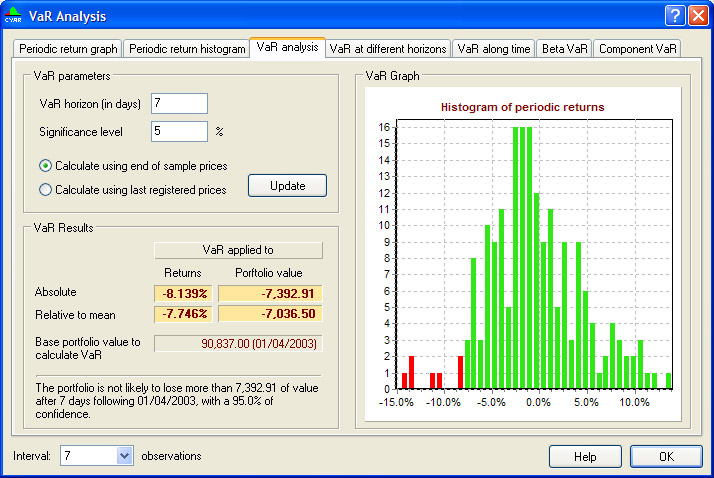
\includegraphics[width=350px]{ecvar_1b.jpg}
			\caption{Vue de \textit{EC-VaR} relative à la VaR caculée selon la méhtode historique}
			\label{ajustement_garch}
		\end{figure}

		Bien qu’il soit probable que l’interface de notre logiciel soit différente, le logiciel ici présenté proche semble le plus proche de notre solution en terme de fonctionnalités, aux méthodes de calcul de la VaR près. % [TODO]: c’est pas sûr ça

		Certains éditeurs ont mis l’accent sur la performance des calculs. C’est le cas de \textit{Quartetfs} qui publie le logiciel \textit{ActivePivot} capable d’un calcul très rapide de la VaR pour un usage en temps réel. Son utilisation se fait à travers une interface web. Il est aussi possible de calculer une VaR marginale, d’analyser les queues de distribution et d’effectuer des simulations de scénarios de stress. Cependant, une telle solution ne correspond pas véritablement à notre besoin : on ne souhaite pas vouloir calculer la VaR pour un usage en temps réel car le modèle de GARCH est mieux adapté pour des prévisions quotidiennes.	Dans la même catégorie, \textit{Mors Software} propose l’add-on \textit{Mors VaR} à ses logiciels existants \textit{Mors liquidity management} et \textit{MORS treasury and trading solutions} pour un calcul performant de la VaR (historique et Monte Carlo). Il possède une fonctionnalité de backtesting. Cependant, l’add-on est une fois de plus orienté vers la performance et ne correspond donc pas au besoin de notre client.

		Parmi les logiciels présentés, il n’en existe finalement aucun capable de calculer directement la VaR selon la méthode GARCH. Un seul est gratuit et aucun n’est libre. Il est probable que les acteurs de la finance intéressés par l’utilisation d’une telle méthode font développer des solutions sur mesure.